\documentclass{sig-alternate-10pt}

\newcommand{\ttt}{\texttt}

\usepackage{graphicx}
\usepackage{changepage}
\usepackage{lipsum}
\usepackage{booktabs}

\title{FLASH\\Fast Linux Advanced Scheduler Hardware}
\author{
	Mark Aligbe \\
	    \email{ma2799@columbia.edu}
	\and
    Chae Jubb \\
        \email{ecj2122@columbia.edu}
}
\date{4 May 2015}

\begin{document}
\maketitle

\begin{abstract}
As accelerators become more common and necessary as a way to continue Moore's Law in the absence of Dennard Scaling, researchers explore segments of computation that can be improved with the aid of dedicated hardware. This paper presents FLASH, a hardware scheduler to take over the task of scheduling from the operating system. FLASH is able to make scheduling decisions in much fewer cycles as compared to modern operating system schedulers. The scheduling decisions it makes are just as good as those that would be made in software, but in much reduced time and without negatively impacting processor performance features. FLASH is designed to keep kernel modifications minimal, only requiring changes when the kernel scheduling interface changes.

\end{abstract}

\section{Introduction}
% \lipsum[1]
Traditional desktop operating systems are interactive, meaning that they serve as the primary interface between a user and a machine. Traditional server operating systems are batch-job oriented, meaning that processes are not pre-empted: a process continues until it exits or is forced to exit due to error. This preemption is one of the performance factors that contribute to greater process utilization on server operating systems as opposed to desktop operating systems. The reason why preemption is detrimental to CPU utilization is a combination of a few different reasons.

\paragraph{TLB and Cache}
The translation lookaside buffer (TLB) is a hardware structure that assists the memory management unit (MMU) of the CPU in translating virtual addresses into physical addresses. The TLB serves as a cache to look up commonly used virtual addresses and return the corresponding physical address. In computationally expensive portions of code, this unit is advantageous as it prevents unnecessary page lookups when the code is accessing a small region of memory. Likewise, the cache on a CPU provides good speedups to this kind of programs, as well as programs that have good data locality.

These structures work very well so long as the same process is in memory. When a context switch, changing from one process to another, is performed, the values of the cache and TLB are essentially invalidated. The new resident process must now wait for expensive memory accesses to bring in valid TLB entries and cache values. Before that process is even loaded, a scheduling algorithm must first decide which process to run next. This results in less than ideal processor utilization.

It is also difficult to make real time scheduling guarantees. In applications such as video playback, it is necessary that the playback process be scheduled consistently to ensure jitter-free playback. FLASH is able to make these guarantees due to its asynchronous computation and throughput. Additionally, FLASH minimizes the penalty to cache and TLB invalidation due to scheduler activity, while providing a complete scheduling interface.

\section{Scheduling in the Kernel}
% Mark
Modern desktop operating systems have to run hundreds of tasks, while providing a responsive interface to the user. This means that the CPU must be able to serve many interrupts a second, from various hardware devices, and service dozens or hundreds of background tasks while presenting a lagless experience to the end user. Each of these sources introduce potential sources of latency: interrupt handling \cite{regehr2007safe} requires many techniques in both hardware and software implementations to maintain relatively cheap and efficient scheduler design is an ongoing field of research \cite{wong2008cfs} \cite{park2008hardware} \cite{morton2004hardware}. We chose to focus on scheduling for our research as the potential benefits of scheduling in hardware in an operating system are not explored in the context of a desktop workload.

\subsection{History of Linux Schedulers}
The linux scheduler has gone through a few major design changes in its scheduler. Before the introduction of the $ O(n) $ scheduler in Linux 2.4, scheduler implementations simple and fast as CPUs themselves had not become as complex as compared to modern CPUs with simultaneous multi-threading (SMT) and symmetric multi-processing (SMP). These implementations were not scalable to multiple processors, so the $ O(n) $ scheduler was introduced to solve the problems introduced by SMP/SMT. The $ O(n) $ scheduler worked well so long as the number of tasks remained low, but as it had a single runqueue for all CPUs in a system, scaled poorly as the number of CPUs grew and as the number of processes grew (since it must iterate through the list of all processes to select a candidate).

The $ O(1) $ scheduler was introduced to solve the problem of large number of tasks. As the name implies, it is able to select a task to run in constant time. The $ O(1) $ scheduler achieves this efficiency by exploiting per-priority \textit{active} and \textit{expired} arrays for tasks. Tasks that are eligible to run are placed in the \textit{active} array and once a task has completed running it is placed in the \textit{expired} array. Thus, selecting a task is as fast as dequeuing the head of the highest priority array. Once the \textit{active} array is empty, the \textit{active} and \emph{expired} arrays are swapped by simply changing pointer directions. Unlike the $ O(n) $ processor, it had per-CPU runqueues, meaning task scheduling did not stall other CPUs. The $ O(1) $ was effective at its job, but was not a fair scheduler, was difficult to maintain through major kernel revisions, and its use of heuristics to determine the interactivity of a process was not without flaw. The CFS scheduler was introduced in Linux 2.6 as a replacement to solve the interactivity issues of the $ O(1) $ scheduler and introduce a simpler, but efficient scheduler.

\subsection{Implementation of CFS}
The CFS scheduler is conceptual simple; it aims to implement an ideal multi-tasking CPU \cite{cfsdesign}.
\subsection{Limitations}


\section{Related Works}
\lipsum[1-2]


\section{FLASH Architecture}
% Chae
\lipsum[1-8]


\section{Integration}
% intro stuff here
\subsection{Cyclone V}
% Mark
\begin{figure}
	\begin{center}
		%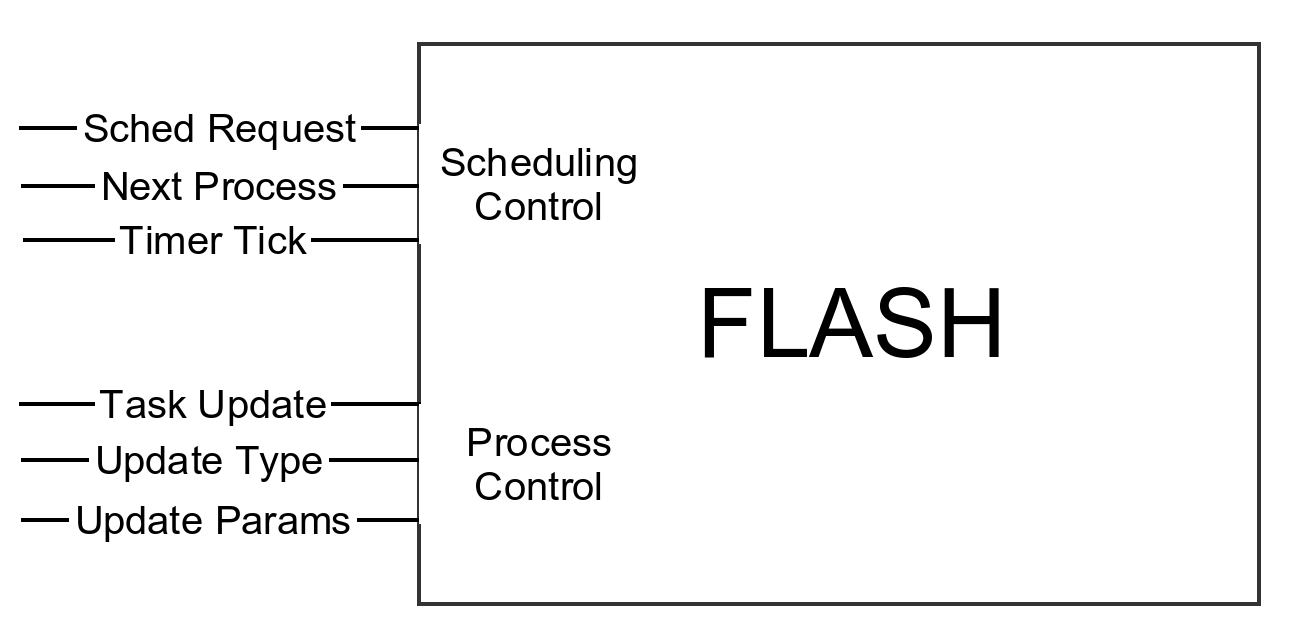
\includegraphics[width=0.65\textwidth]{fig/flash-diagram.png}
		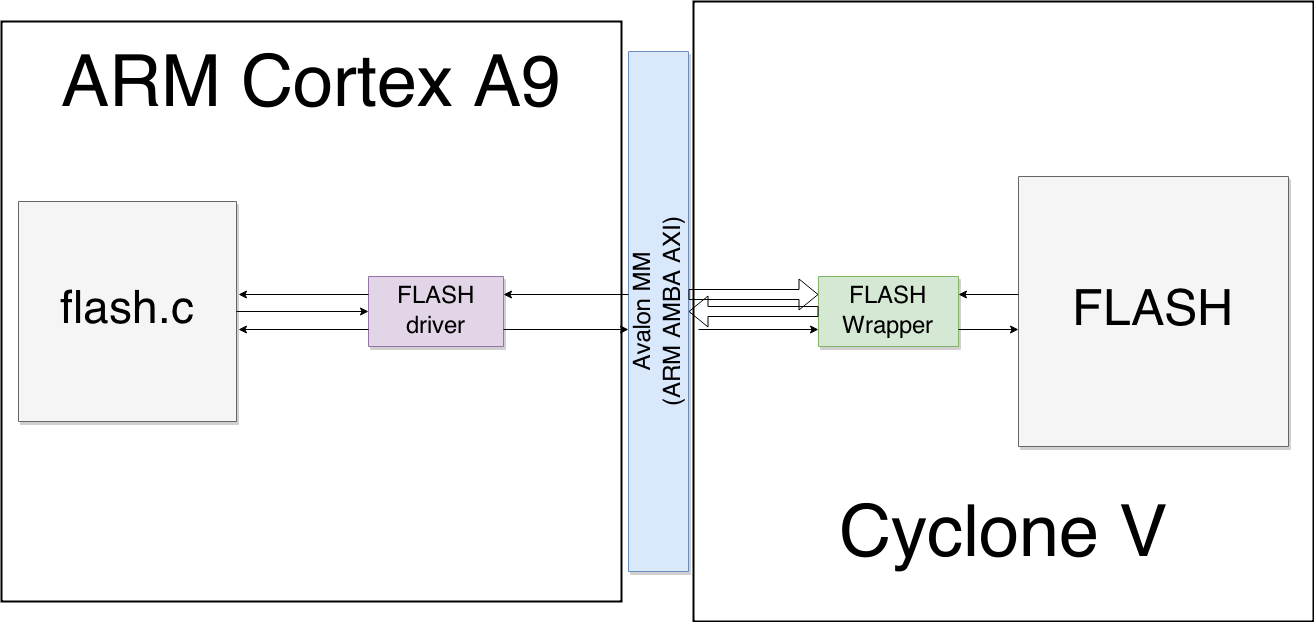
\includegraphics[width=0.9\linewidth]{fig/sockit-architecture.png}
		\caption{
			Arrow SoCKiT high level overview. The embedded ARM processor is connected to the FPGA fabric via a ARM's AMBA AXI interface, on top of which runs Altera's Avalon MM interface.
		}
		\label{fig:sockit_overview}
	\end{center}
\end{figure}


\subsection{Kernel mods}
% Chae
\lipsum[1-3]


\section{Applications}
% Mark
\lipsum[1-3]


\section{Engineering Experiences}
% both
\lipsum[1-3]

\section{Future Work}
\subsection{DMA}
\subsection{No HZ Interrupt}

\section{Conclusion}
\lipsum[1]

\nocite{*}
{
	\bibliographystyle{abbrv}
	\bibliography{ref}
}

\end{document}
